% !TEX root = hazelnut-popl17.tex
\subsection{Implementation Concepts}
Central to any implementation of Hazelnut is a stream of edit states whose
cursor erasures synthesize types under an empty context according to the
synthetic action judgement,
$\performSyn{\emptyset}{\zexp}{\htau}{\alpha}{\zexp'}{\htau'}$. The middle
row of Figure \ref{fig:impl-overview} diagrams this stream of edit
states. For example, the reader is encouraged to re-examine the
examples in Figure \ref{fig:first-example} and \ref{fig:second-example} --
the cursor erasure of each edit state synthesizes a type.


Because Theorem \ref{thrm:actsafe} expresses an invariant, the editor does not need to
typecheck the edit state anew on each action (though in some of the rules, e.g. Rule
(\ref{rule:zipper-asc}) which handles the situation where the type in a
type ascription changes, portions of the program would need to be
typechecked again.) In other words, many of the problems related to incrementality 
are simply not relevant. Storing the types of subtrees would allow for further
optimizations (e.g. of the zipper rules.)

The programmer examines a view generated from each edit state and produces
actions in some implementation-defined manner (e.g. using a keyboard,
mouse, touchscreen, voice interface, or neural interface), as diagrammed in Figure \ref{fig:impl-overview}. Each new action
causes a new abstract edit state to arise according to an implementation of
the action semantics. This then causes a new view to arise. This is a
simple event-based functional reactive programming model
\cite{Wan:2000:FRP:349299.349331}.

If an action is not well-defined according to Hazelnut's action semantics,
the implementation must reject it. In fact, the implementation is
encouraged to present an ``action palette'' that either hides or visibly
disables actions that are not well-defined (see below.)

\begin{figure}
\centering
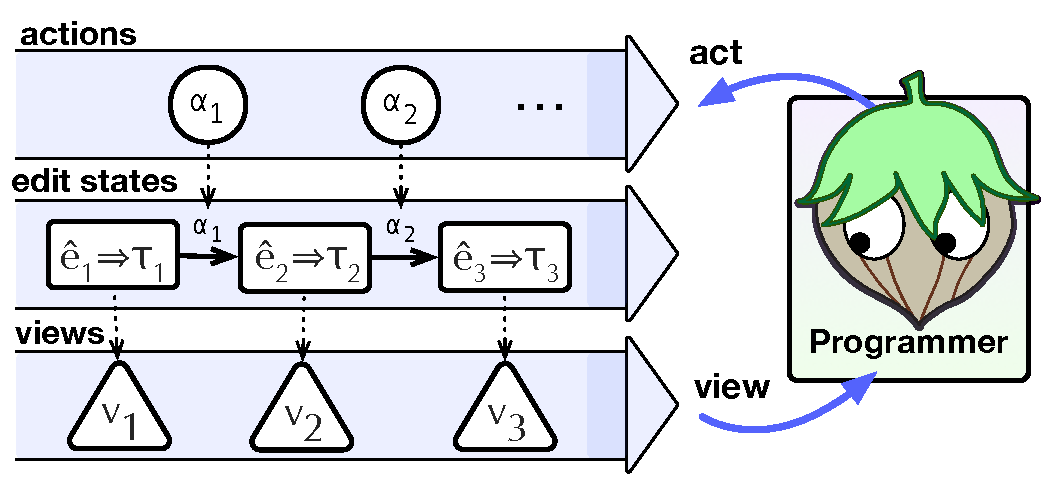
\includegraphics[width=\columnwidth]{impl-overview2}
\caption{Implementation Concepts}
\label{fig:impl-overview}
\end{figure}

\subsection{HZ}
We have developed a simple reference implementation, HZ, of Hazelnut extended with sum types as described in Sec. \ref{sec:extending}.  In
order to reach a wide audience, we decided to implement HZ in the web
browser.  To take advantage of a mature implementation of the FRP
model, we chose to implement HZ using
OCaml\footnote{\url{https://ocaml.org/}}, the \texttt{js\_of\_ocaml}
compiler and associated libraries
\cite{DBLP:conf/ml/Balat06}\footnote{\url{http://ocsigen.org/js\_of\_ocaml/}}
and the OCaml React
library\footnote{\url{http://erratique.ch/software/react}}.

The core semantics have
been implemented in a functional style that follows the presentation in this paper closely.

The view computation renders the model (i.e. a Z-expression paired with a type) as nested HTML \texttt{div} elements matching the tree structure of the corresponding Z-expression. This tree is stylized separately using CSS. The action palette is a collection of buttons and text boxes which
are disabled when the corresponding action cannot be performed. We determine this by simply attempting to perform the
action internally and handling the exception that is raised when an action
is undefined. (An optimization that is not in HZ would be to implement a version of the action semantics that simply computes a boolean, rather than the resulting edit state, for the purposes of action validation.) Each action form also has a corresponding keyboard shortcut. For actions that take arguments, the keyboard shortcut moves the cursor into a text box. The action validation occurs on every change to the text box.

This implementation is not, of course, meant to score marks for
usability or performance (though both are surprisingly good for such a simple system.) Instead, as a simple reference implementation, it allows the reader to interact with the system presented in this paper, to aid in their understanding.  Additionally, we expect its source code to be of use to others who are interested in
layering a more fluid user interface atop the core semantics, or extensions thereof. 
